\documentclass[10pt,a4paper]{article}
\usepackage[a4paper,margin=25mm]{geometry}
% Compilar com pdfLaTeX e Biber.
\usepackage[T1]{fontenc}
\usepackage[utf8]{inputenc}
\usepackage[sfdefault,type1]{arimo}
\usepackage[portuguese]{babel}
\usepackage{graphicx,booktabs,tabularx,array,xcolor,colortbl,caption,subcaption,csquotes}
% Estilo bibliográfico de escolha livre. A configuração seguinte é apenas um exemplo.
% Para APA, por exemplo, substituir a linha por:
% \usepackage[backend=biber,style=apa]{biblatex}
% Para IEEE, se disponível, utilizar style=ieee. Ajustar as opções ao estilo escolhido.
\usepackage[backend=biber,sorting=none,style=numeric-comp]{biblatex}
\addbibresource{referencias.bib}
\definecolor{azul}{RGB}{20,20,150}
\usepackage{mathtools,amssymb,bm}
\usepackage{titlesec}
\titleformat{\section}{\fontsize{12bp}{14bp}\selectfont\bfseries\color{azul}}{\thesection}{0.6em}{}
\titleformat{\subsection}{\fontsize{11bp}{13bp}\selectfont\bfseries\color{azul}}{\thesubsection}{0.6em}{}
\titleformat{\subsubsection}{\fontsize{10bp}{12bp}\selectfont\bfseries}{\thesubsubsection}{0.6em}{}
\titlespacing*{\section}{0pt}{12bp}{6bp}
\titlespacing*{\subsection}{0pt}{10bp}{4bp}
\titlespacing*{\subsubsection}{0pt}{10bp}{4bp}
\setlength{\parindent}{0pt}
\setlength{\parskip}{6bp}
\captionsetup{font=small}
\AtBeginDocument{\fontsize{10bp}{11.5bp}\selectfont}
\makeatletter
\renewcommand\normalsize{\@setfontsize\normalsize{10bp}{11.5bp}}
\renewcommand\small{\@setfontsize\small{9bp}{10.5bp}}
\makeatother

\usepackage[colorlinks=true,allcolors=azul]{hyperref}
\numberwithin{equation}{section}
\newcommand{\orientacao}[1]{\par\noindent{\normalsize\itshape\color{black!65}#1}\par}
% Substituir os campos seguintes.
\newcommand{\tituloPT}{Aquisição e Estruturação de Dados Multimodais de Precisão de Pomares}
\newcommand{\tituloEN}{Acquisition and Structuring of High-Precision Multimodal Data from Orchards}
\newcommand{\tipologia}{[Dissertação / Projeto / Estágio]}
\newcommand{\estudante}{Marco António Aparício Pereira}
\newcommand{\numero}{130641}
\newcommand{\orientadores}{Daniela Rato e Vítor Santos}
\newcommand{\dataentrega}{[Data de entrega]}
\usepackage{siunitx,forloop}
\newcounter{loopcntr}
\newcommand{\rpt}[2][1]{%
  \forloop{loopcntr}{0}{\value{loopcntr}<#1}{#2}%
}
\newcommand{\on}[1][1]{
  \forloop{loopcntr}{0}{\value{loopcntr}<#1}{&\cellcolor{orange}}
}
\newcommand{\onM}[1][1]{
  \forloop{loopcntr}{0}{\value{loopcntr}<#1}{&\cellcolor{gray}}
}
\newcommand{\off}[1][1]{
  \forloop{loopcntr}{0}{\value{loopcntr}<#1}{&}
}

\begin{document}


\begin{titlepage}
\centering
{\large Universidade de Aveiro\\ Departamento de Engenharia Mecânica\\ Mestrado em Engenharia Mecânica\par}
\vspace{1cm}
{\large Metodologias de Apoio à Opção DPE (49688)\\ 2026/2027\par}
\vfill
{\color{azul}\LARGE\bfseries Enquadramento Técnico-Científico\par}
\vspace{1cm}
{\Large\bfseries\tituloPT\par}
\medskip
{\large\tituloEN\par}
\medskip
{\large\tipologia\par}
\vfill
{\large\estudante\ --- \numero\par}
\medskip
Orientação: \orientadores\par
\vfill
\dataentrega
\end{titlepage}


\pagenumbering{roman}

\section*{Resumo}
\orientacao{Apresentar, de forma sucinta, o tema, o âmbito da revisão, os principais aspetos analisados e as conclusões decorrentes da análise crítica do conhecimento existente. Extensão sugerida: 150 a 250 palavras.}
\section*{Palavras-chave}
\orientacao{Indicar entre três e cinco palavras-chave representativas do tema e do conteúdo do documento.}
\clearpage
\section*{Reconhecimento do uso de ferramentas IA}
Reconheço o uso de \textit{[inserir sistema(s) de IA e respetiva hiperligação]} para \textit{[indicar utilização específica de IA ou outras tarefas]}. Reconheço a utilização de \textit{[indicar software, código ou plataforma]} para \textit{[indicar utilização específica de software, código ou plataforma ou para outras tarefas]}.

\medskip
\orientacao{Exemplo 1: Reconheço a utilização do ChatGPT 3.5 (Open AI, \url{https://chat.openai.com}) para resumir as notas iniciais e para rever o rascunho final, a utilização do Office365 (Microsoft, \url{https://www.office.com}) para a escrita do texto.}

\orientacao{Exemplo 2: Não foram utilizados no presente trabalho quaisquer conteúdos gerados por tecnologias de IA.}

\orientacao{O estudante deverá adaptar a declaração à utilização efetiva das tecnologias e ferramentas de apoio, eliminando os exemplos e os textos orientadores na versão de entrega.}
\clearpage

\tableofcontents
\clearpage
\pagenumbering{arabic}
\orientacao{Máximo de 15 páginas úteis, excluindo capa, resumo, palavras-chave, declaração de utilização de IA e ferramentas de apoio, índice e referências bibliográficas. Sem limite de referências bibliográficas. Não são admitidos anexos ou apêndices. Respeitar a formatação do template (Arimo (metricamente compatível com Arial), 10 pt, espaçamento simples e margens de 25 mm). Os textos orientadores estão em itálico e a cinzento. O texto Lorem ipsum exemplifica a formatação do corpo do documento (preto, sem itálico). Eliminar ambos na versão de entrega.}
\orientacao{A estrutura apresentada neste template é meramente indicativa. O estudante deverá definir a organização do documento, incluindo a designação, o número e a sequência das secções e subsecções, em função da natureza, da especificidade e dos objetivos da Dissertação, Projeto ou Estágio.}
\orientacao{Independentemente da estrutura adotada, o documento deverá contemplar a contextualização do tema, a revisão e análise crítica do conhecimento relevante e o posicionamento do trabalho a desenvolver. As figuras e tabelas são meramente exemplificativas, tanto na estrutura como no conteúdo, e não são de inclusão obrigatória.}

\section{Introdução e âmbito da revisão}
\orientacao{Contextualizar o tema da D/P/E e delimitar o âmbito da revisão técnico-científica. Identificar os principais aspetos a aprofundar e justificar a sua relevância para o trabalho a desenvolver.}

Lorem ipsum dolor sit amet, consectetur adipiscing elit. Sed do eiusmod tempor incididunt ut labore et dolore magna aliqua. Ut enim ad minim veniam, quis nostrud exercitation ullamco laboris nisi ut aliquip ex ea commodo consequat. Duis aute irure dolor in reprehenderit in voluptate velit esse cillum dolore eu fugiat nulla pariatur.


\section{Enquadramento técnico-científico e análise crítica}
\orientacao{Apresentar, discutir e analisar criticamente os conceitos, fundamentos, conhecimentos, soluções, metodologias, tecnologias ou práticas relevantes para o trabalho, sustentando a discussão em fontes bibliográficas relevantes e credíveis. Identificar, quando aplicável, vantagens, limitações, lacunas e oportunidades, fundamentando o posicionamento do trabalho a desenvolver.}
\orientacao{Organizar o conteúdo em secções e/ou subsecções temáticas, de acordo com a natureza e a especificidade da D/P/E. A análise crítica e o posicionamento do trabalho poderão ser desenvolvidos de forma integrada ou em secções autónomas, consoante a organização considerada mais adequada pelo estudante.}

Lorem ipsum dolor sit amet, consectetur adipiscing elit. Sed do eiusmod tempor incididunt ut labore et dolore magna aliqua. Ut enim ad minim veniam, quis nostrud exercitation ullamco laboris nisi ut aliquip ex ea commodo consequat. Duis aute irure dolor in reprehenderit in voluptate velit esse cillum dolore eu fugiat nulla pariatur.


% Exemplo de equação: eliminar ou adaptar na versão de entrega.
\orientacao{Quando aplicável, as equações deverão ser numeradas, referenciadas no texto e acompanhadas da identificação das grandezas e parâmetros envolvidos. O exemplo seguinte é meramente ilustrativo; a inclusão de equações não é obrigatória.}
\orientacao{A Equação~\eqref{eq:hooke} representa a lei de Hooke no regime elástico linear uniaxial.}
\begin{equation}
  \sigma = E\varepsilon
  \label{eq:hooke}
\end{equation}
\orientacao{Nesta expressão, $\sigma$ representa a tensão normal, $E$ o módulo de Young e $\varepsilon$ a deformação longitudinal.}

% Exemplo de figura: eliminar ou substituir na versão de entrega.
\orientacao{Todas as figuras devem ser referidas no texto e acompanhadas de uma legenda descritiva, indicando a fonte quando aplicável. A Figura~\ref{fig:T2fig} apresenta um exemplo de inserção e referenciação de uma figura.}
\begin{figure}[!htb]
\centering
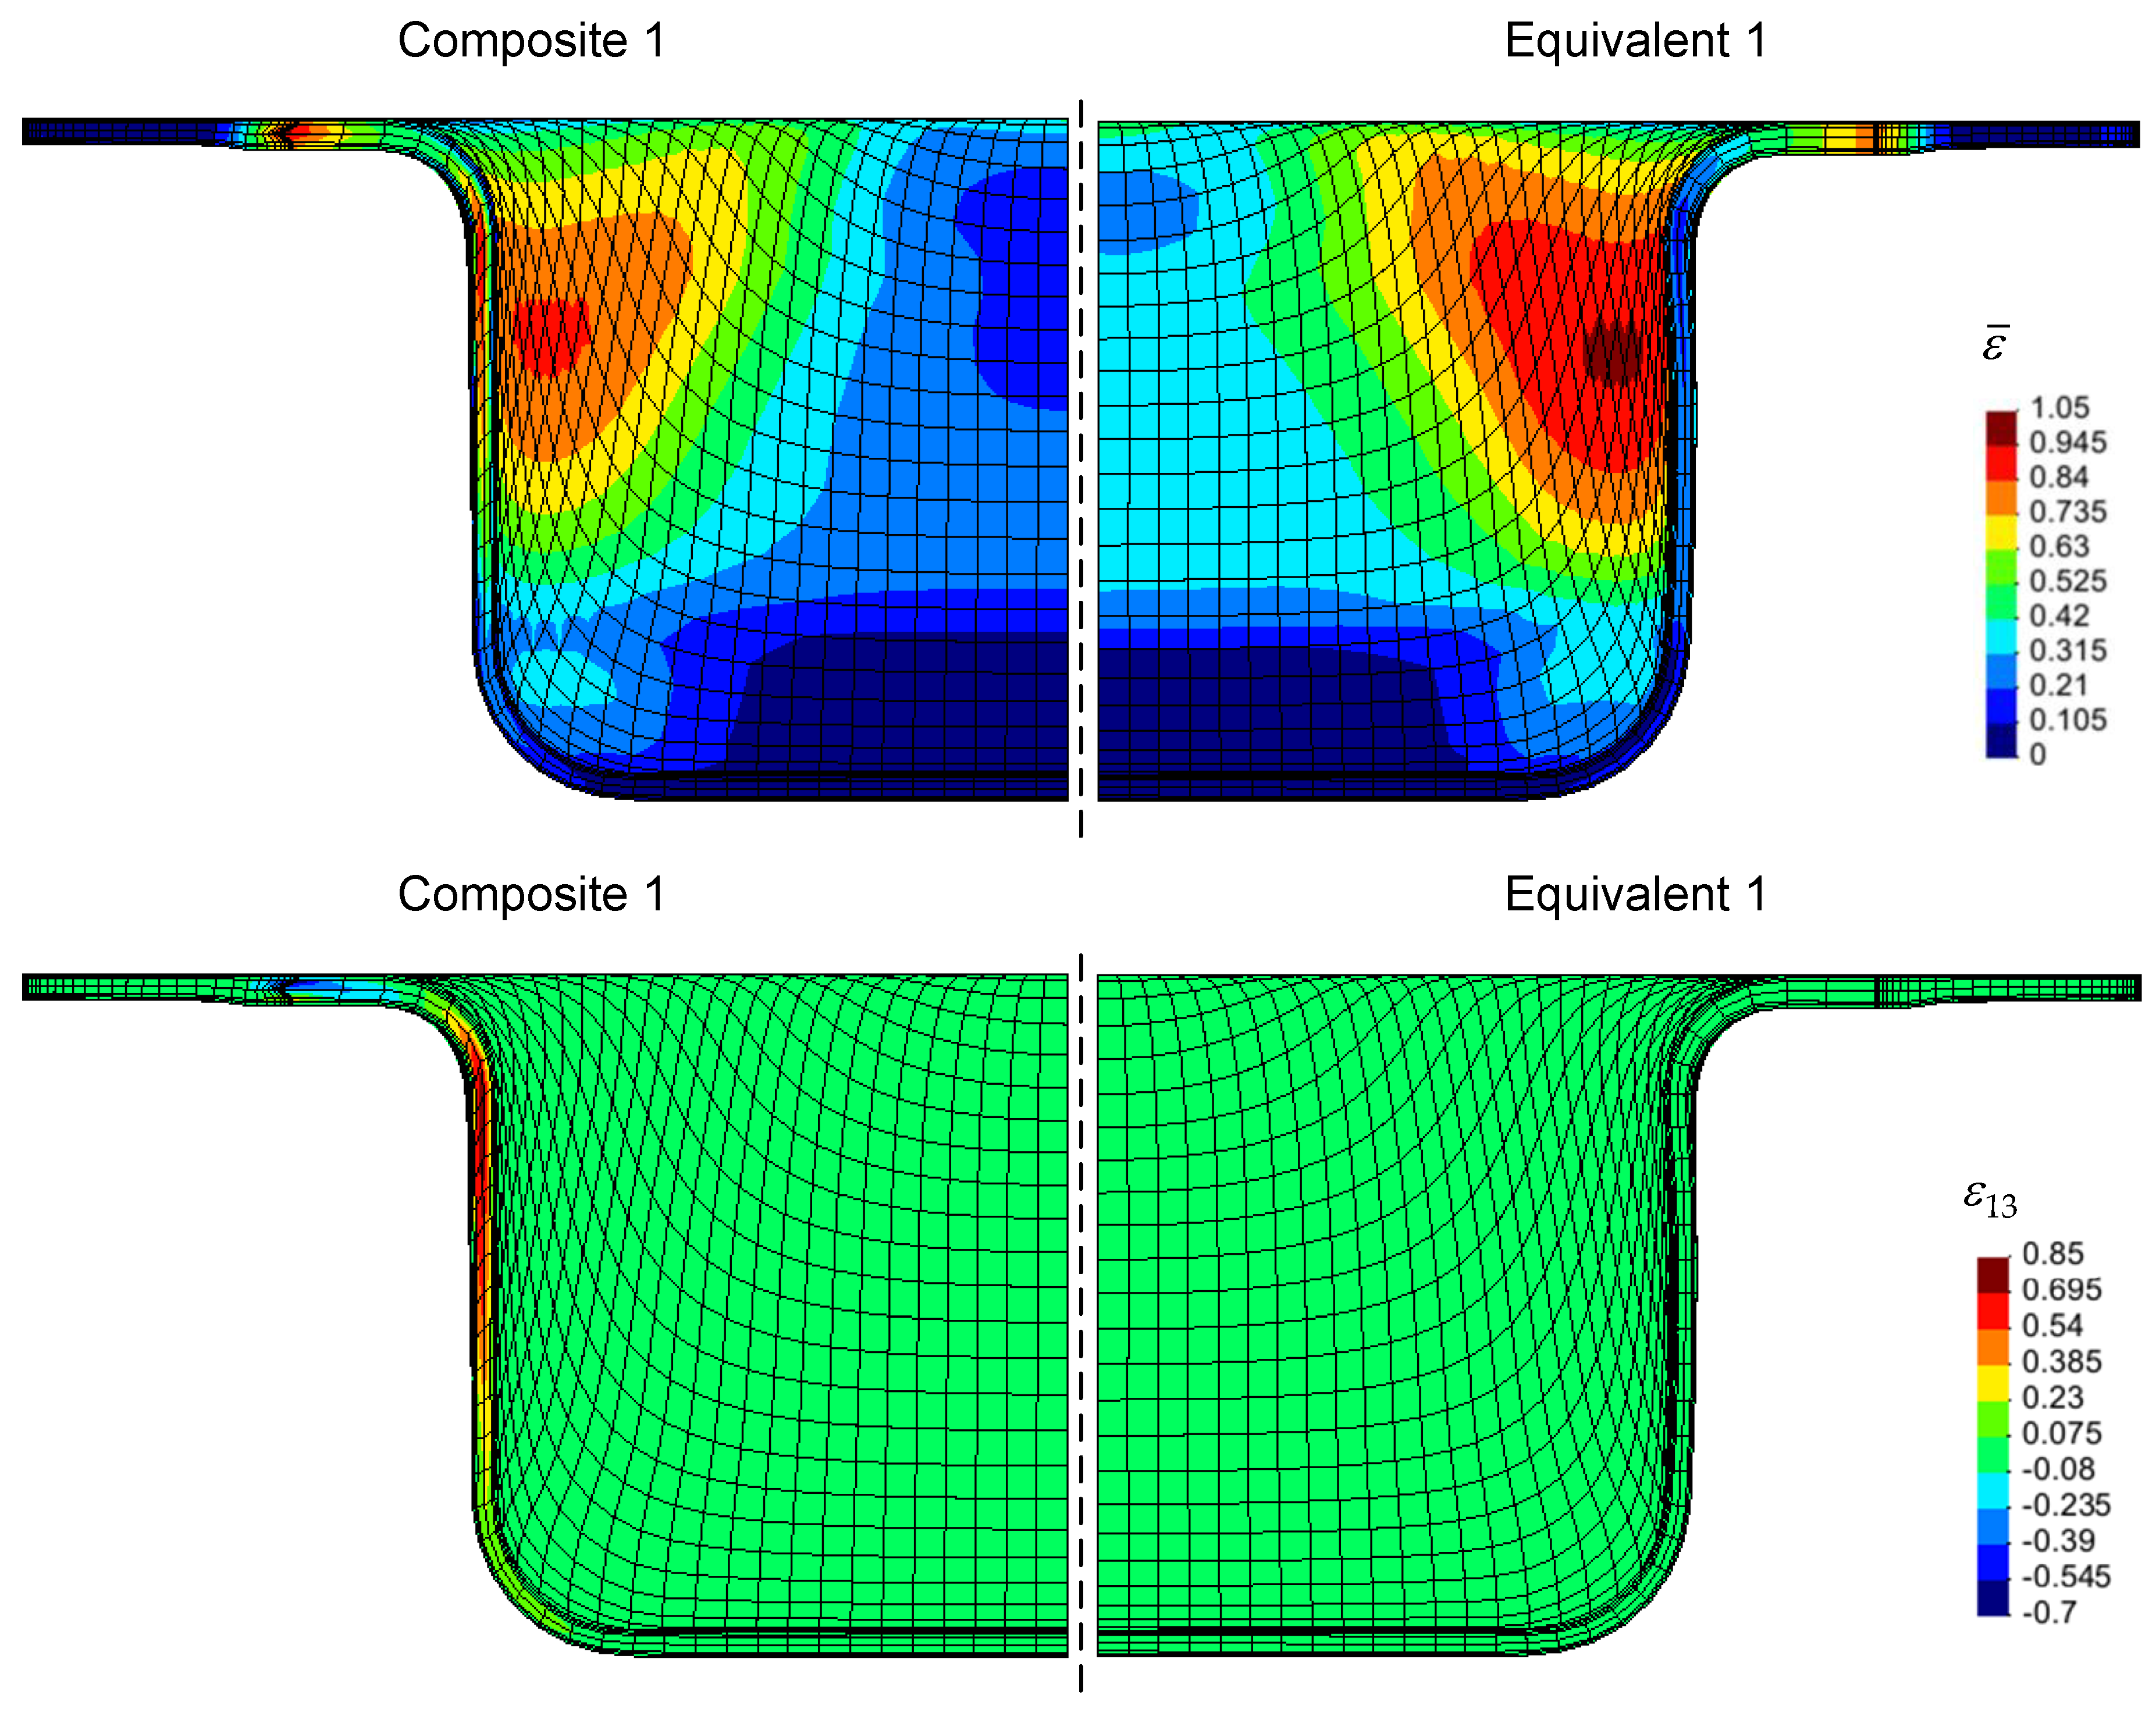
\includegraphics[width=0.65\linewidth]{pics/Fig1.png}
\caption{Exemplo de figura 1.}
\label{fig:T2fig}
\end{figure}
\orientacao{A Tabela~\ref{tab:exemplo} exemplifica a comparação crítica da literatura. A tabela é meramente exemplificativa, tanto na sua estrutura como no seu conteúdo. A utilização de tabelas de síntese ou de análise comparativa e a definição dos respetivos critérios deverão ser adequadas à natureza do tema e aos objetivos da revisão. Caso seja utilizada, deverá basear-se em trabalhos efetivamente consultados e citados. As legendas das tabelas devem ser colocadas acima das mesmas.}
\begin{table}[!htb]
\centering
\caption{Exemplo ilustrativo de uma tabela de análise comparativa da literatura.}
\label{tab:exemplo}
\normalsize
\renewcommand{\arraystretch}{1.2}
\begin{tabularx}{\linewidth}{@{}*{4}{>{\raggedright\arraybackslash}X}@{}}
\toprule
\textbf{Referência} & \textbf{Metodologia} & \textbf{Principais contributos} & \textbf{Limitações} \\
\midrule
Estudo A & Modelação analítica & Reduzido custo computacional & Hipóteses simplificativas \\
Estudo B & Simulação numérica & Flexibilidade de aplicação & Elevado custo computacional \\
Estudo C & Abordagem experimental & Validação em condições reais & Aplicabilidade limitada \\
\bottomrule
\end{tabularx}
\end{table}

\clearpage

\phantomsection
\section*{Referências bibliográficas}
\addcontentsline{toc}{section}{Referências bibliográficas}
\orientacao{Incluir todas as fontes citadas ao longo do documento, privilegiando fontes científicas e técnicas relevantes e credíveis. O estilo de referenciação bibliográfica (IEEE, APA, entre outros) é de escolha livre, devendo ser utilizado de forma consistente ao longo de todo o documento. O estilo apresentado neste template é meramente exemplificativo e não tem caráter vinculativo. Todas as referências devem ser citadas no texto. Não existe limite para o número de referências bibliográficas.}
\orientacao{Exemplos de citação individual \cite{einstein:1905} e múltipla \cite{dirac:1981,knuthwebsite:2016}. Eliminar estes exemplos na versão de entrega.}
\printbibliography[heading=none]

\end{document}
